\documentclass{beamer}
\usepackage[latin1]{inputenc,colortbl}
\usepackage{epsfig}
\usetheme{Frankfurt}
\setbeamertemplate{navigation symbols}{}
\setbeamertemplate{footline}[page number]
%\newtheorem{definition}{Definition}
\title[Lecture 8: Coalition Games]{Lecture 8: Coalition Games}
\author{INSE 6441/2\\ \vspace{0.2cm} Applied Game Theory and Mechanism Design}
\institute{Department of Computer Science and Software Engineering\\Concordia University}
\date{Ehsan Khosrowshahi \\ \small{Acknowledgement: Stephane Airiau, Lloyd Shapley}}
\begin{document}
%%%%%%%%%%%%%%%%%%%%%%%%%%%%%%%% frame1 title page %%%%%%%%%%%%%%%%%%%%%%%%%%%%%%%%%%%%%%%
%%%%%%%%%%%%%%%%%%%%%%%%%%%%%%%%%%%%%%%%%%%%%%%%%%%%%%%%%%%%%%%%%%%%%%%%%%%%%%
\begin{frame}
\titlepage
\end{frame}
%%%%%%%%%%%%%%%%%%%%%%%%%%%%%%%% frame2 outline page %%%%%%%%%%%%%%%%%%%%%%%%%%%%%%%%%%%%%
%%%%%%%%%%%%%%%%%%%%%%%%%%%%%%%%%%%%%%%%%%%%%%%%%%%%%%%%%%%%%%%%%%%%%%%%%%%%%%

\begin{frame}{Overview}
    \begin{itemize}
     	\itemsep=.5cm
    	\item {\bf Coalition Games}
    	\item Stability and Core
    	\item Fairness and Shapley Value
    	\item Other Solution Concepts
        \item Practical Example
    \end{itemize}
\end{frame}


%%%%%%%%%%%%%%%%%%%%%%%%%%%%%%%%%%%%%%%%%%%%%%%%%%%%%%%%%%%%%%%%%%%%%%%%%%%%%%
\section{Coalition Games}
\subsection{Cooperative Game Theory}

\begin{frame}{Cooperative Game Theory}
  \begin{itemize}
     \item In game theory, a cooperative game is a game where groups of players $``coalitions''$ may enforce cooperative behaviour, hence the game is a competition between coalitions of players, rather than between individual players.
    \item Cooperation to perform a set of tasks that requires different expertise.
    \item Agents do not have enough resource on their own to perform the tasks.
    \item Examples:
    \begin{itemize}
        \item Robots have the ability to move objects in a plant, but multiple robots are required to move a heavy box.
        \item Transportation domain: agents are trucks, trains, airplanes, ships... a task is a good to be transported.
    \end{itemize}
    \item \textbf{Issues:}
        \begin{itemize}
            \item Coalition formation.
            \item Rewarding members when a task is completed.
        \end{itemize}
  \end{itemize}
\end{frame}

%%%%%%%%%%%%%%%%%%%%%%%%%%%%%%%% frame14 Background and Literature Review %%%%%%%%%%%%%%%%%%%%%%%%%%%%%%%%%%%%%
%%%%%%%%%%%%%%%%%%%%%%%%%%%%%%%%%%%%%%%%%%%%%%%%%%%%%%%%%%%%%%%%%%%%%%%%%%%%%%
\begin{frame}{Cooperative Game Theory}
    \begin{itemize}
         \item Cooperative games are a branch of game theory that models cooperation or collaboration between agents within coalitions.
    \end{itemize}
    \begin{definition} [Coalition]~\\
       We have a population $N$ of $n$ agents, A coalition $C$ is a set of agents: $C \in 2^N$.
        \begin{itemize}
            \item $N$ is the set of all agents (or players)
            \item $v:2^N \rightarrow R$ is the \emph{valuation function}. For $C \subseteq N$, $v(C)$ is the value obtained by the coalition $C$
        \end{itemize}
    \end{definition}

    \begin{itemize}
        \item \textbf{Problem:} Given a game $(N,v)$, and assuming all agents in $N$ want to cooperate, how to distribute the gain among the agents?
        \item \textbf{Solution:} a payoff distribution $x \in R^n$ that provides a value to individual agents.

        \begin{itemize}
            \item What are the interesting properties that $x$ should satisfy?
            \item How to determine the payoff vector $x$?
        \end{itemize}

    \end{itemize}
\end{frame}
%%%%%%%%%%%%%%%%%%%%%%%%%%%%%%%%%%%%%%%%%%%%%%%%%%%%%%%%%%%%%%%%%%%%%%%%%%%%%%

\begin{frame}{An Example}

    \begin{center}
        $N = \{1,2,3\}$ \\
        $v(\{1\}) = 0, v(\{2\}) = 0, v(\{3\}) = 0$ \\
        $v(\{1,2\}) = 90$ \\
        $v(\{1,3\}) = 80$ \\
        $v(\{2,3\}) = 70$ \\
        $v(\{1,2,3\}) = 105$ \\
    \end{center}

    What should we do?
    \begin{itemize}
        \item form $\{1,2,3\}$ and share equally $(35,35,35)$?
        \item 3 can say to 1 ``let's form $\{1,3\}$ and share (40,0,40)''
        \item 2 can say to 1 ``let's form $\{1,2\}$ and share (45,45,0)''
        \item 3 can say to 2 ``OK, let's form $\{2,3\}$ and share (0,46,24)''
        \item 1 can say to 2 and 3, ``fine! $\{1,2,3\}$ and (33,47,25)''
        \item ...what is a good solution?
    \end{itemize}

\end{frame}

%%%%%%%%%%%%%%%%%%%%%%%%%%%%%%%% frame15 outline page

%%%%%%%%%%%%%%%%%%%%%%%%%%%%%%%%%%%%%%%%%%%%%%%%%%%%%%%%%%%%%%%%%%%%%%%%%%%%%%
\begin{frame}{Transferable and Non Transferable Utility Games}
    \begin{itemize}
        \item \textbf{Games with Transferable Utility (TU games)}
        \begin{itemize}
            \item Utility is worth the same for all agents.
            \item Utility can be {\color{red} compared} or {\color{red} transferred} between agents.
            \item Irrespective of the division of the coalitional payoff.
            \begin{itemize}
                \item In that case members of the coalition enjoy the same total utility.
            \end{itemize}
        \end{itemize}


        \begin{definition} [Valuation or Characteristic Function]\label{dfn:valuationfunction}
            A \emph{valuation function v} associates a real number $v(C)$ to any subset $C \subseteq N$, i.e., $v:2^N \rightarrow R$ \\
            A {\color{blue}\emph{TU game}} is a pair $(N,v)$ where $N$ is a set of agents and where $v$ is a valuation function.
        \end{definition}



        \item \textbf{Games with Non Transferable Utility (NTU games)} \\
            Agents have different preferences over coalitions and rewards. Non-monetary rewards, i.e. item allocation type of problems where items have different values for different players.
    \end{itemize}
\end{frame}

%%%%%%%%%%%%%%%%%%%%%%%%%%%%%%%%%%%%%%%%%%%%%%%%%%%%%%%%%%%%%%%%%%%%%%%%%%%%%%%
\begin{frame}{Some Properties of Valuation Functions}
    $\forall C_1,C_2 \subseteq N | C_1 \bigcap C_2 = \emptyset, i \in N, i \notin C_1$
    \begin{itemize}
        \item {\color{blue} Additive:} $v(C_1 \bigcup C_2) = v(C_1) + v(C_2)$
        \item {\color{blue} Super additive:} $v(C_1 \bigcup C_2) \geq v(C_1) + v(C_2)$ This is satisfied is many applications, or bigger coalitions will not form.
        \item {\color{blue} Weekly super additive:} $v(C_1 \bigcup \{i\}) \geq v(C_1) + v(\{i\})$
        \item {\color{red} Subadditive:} $v(C_1 \bigcup C_2) \leq v(C_1) + v(C_2)$
    \end{itemize}

    $\forall C_1,C_2 \subseteq N$
    \begin{itemize}
        \item {\color{blue} Convex:} $v(C_1 \bigcup C_2) \geq v(C_1) + v(C_2) - v(C_1 \bigcap C_2)$. Convexity has important properties in cooperative game theory solution concepts.
    \end{itemize}

    $\forall C \subseteq S \subseteq N$
    \begin{itemize}
        \item {\color{blue} Monotonic:} $v(C) \leq v(S)$
    \end{itemize}
\end{frame}
%%%%%%%%%%%%%%%%%%%%%%%%%%%%%%%%%%%%%%%%%%%%%%%%%%%%%%%%%%%%%%%%%%%%%%%%%%%%%%
\begin{frame}{Solution Properties}
    Let $x \in R^n$ be a solution of the coalition game $(N,v)$
    \begin{itemize}
        \item {\color{blue} Feasible solution:} $\sum_{i \in N} x(i) \leq v(N)$
        \item {\color{blue} Efficiency:} $\sum_{i \in N} x(i) = v(N)$
        \begin{itemize}
            \item the payoff distribution is an allocation of the entire worth of the grand coalition to all agents.
        \end{itemize}
        \item {\color{blue} Individual rationality:} $\forall i \in N, x(i) \geq v(\{i\})$
        \begin{itemize}
            \item player obtains at least its self-value of payoff.
        \end{itemize}
    \end{itemize}

\end{frame}

%%%%%%%%%%%%%%%%%%%%%%%%%%%%%%%%%%%%%%%%%%%%%%%%%%%%%%%%%%%%%%%%%%%%%%%%%%%%%%
\begin{frame}{Solution Properties (Cont.)}
    Let $x \in R^n$ be a solution of the coalition game $(N,v)$
    \begin{itemize}
        \item {\color{blue} Group rationality:} $\forall C \subseteq N, \sum_{i \in N} x(i) \geq v(C)$
        \begin{itemize}
            \item if $\sum_{i \in N} x(i) < v(C)$ is not worth it for some $C$
            \item if $\sum_{i \in N} x(i) > v(C)$ is not possible for all $C$
        \end{itemize}
%        \item {\color{blue} Pareto Optimal:} $\sum_{i \in N} x(i) = v(N)$
%        \begin{itemize}
%            \item no agent can improve its payoff without lowering the payoff of another agent
%        \end{itemize}
        \item {\color{blue} Anonymity:} a solution is independent of the names of the player.
    \end{itemize}

    \vspace{0.2cm}

    An {\color{blue} imputation} is a payoff distribution $x$ that is efficient and individual rational.

\end{frame}
%%%%%%%%%%%%%%%%%%%%%%%%%%%%%%%%%%%%%%%%%%%%%%%%%%%%%%%%%%%%%%%%%%%%%%%%%%
%%%%%%%%%%%%%%%%%%%%%%%%%%%%%%%%%%%%%%%%%%%%%%%%%%%%%%%%%%%%%%%%%%%%%%%%%%
\section{Stability and Core}
\subsection{Stability and Core}

%%%%%%%%%%%%%%%%%%%%%%%%%%%%%%%%%%%%%%%%%%%%%%%%%%%%%%%%%%%%%%%%%%%%%%%%%%
\begin{frame}{Overview}
    \begin{itemize}
     	\itemsep=.5cm
    	\item Coalition Games
    	\item {\bf Stability and Core}
    	\item Fairness and Shapley Value
    	\item Other Solution Concepts
        \item Practical Example
    \end{itemize}
\end{frame}

%%%%%%%%%%%%%%%%%%%%%%%%%%%%%%%%%%%%%%%%%%%%%%%%%%%%%%%%%%%%%%%%%%%%%%%%%%
\begin{frame}{Stability}
    \begin{itemize}
        \item We all want to work together and get $v(N)$, but we all have different views about how to share the fruits of our work. We can use the values of other coalitions as arguments in favor of a distribution.
        \item A condition for a coalition to form:
            {\color{blue}all} agents prefer to be in it. i.e., none of the participants wishes she were in a different coalition or by herself {\color{blue} $\Rightarrow Stability$ }
        \item The {\color{blue} core} is a stability concept for which no agents prefer to deviate to form a different coalition.
    \end{itemize}
\end{frame}

%%%%%%%%%%%%%%%%%%%%%%%%%%%%%%%%%%%%%%%%%%%%%%%%%%%%%%%%%%%%%%%%%%%%%%%%%%%%%%
\begin{frame} {Solution Concepts: Core}
    The core relates to the stability of the grand coalition: \\ No group of agents has any incentive to change coalition.
    \begin{definition}[$Core$ of a Game $(N,v)$]\label{dfn:core}
        Let $(N,v)$ be a cooperative game, and assume they form the coalition $N$. The core of $(N,v)$ is the set:
        \vspace{0.1cm}
        \begin{center}
            $Core(N,v) = \{x \in R^n | x$ is a group rational imputation$\}$
        \end{center}
        Equivalently,
        \vspace{0.1cm}
        \begin{center}
            $Core(N,v) = \{x \in R^n | x(N) \leq v(N) \wedge x(C) \geq v(C), \forall C \subseteq N\}$ \\
        \end{center}
        \small{$x(N) = \sum_{i \in N} x(i)$}
    \end{definition}

    \begin{itemize}
       \item The coalition is stable $\Leftrightarrow$ The core is not empty
    \end{itemize}

\end{frame}
%%%%%%%%%%%%%%%%%%%%%%%%%%%%%%%%%%%%%%%%%%%%%%%%%%%%%%%%%%%%%%%%%%%%%%%%%%%%%%
\begin{frame} {Example 1: A two-player game}

    \begin{center}
      $N = \{1,2\}$ \\
      $v(\{1\}) = 5, v(\{2\}) = 5$ \\
      $v(\{1,2\}) = 20$ \\
    \end{center}

    $Core(N,n) = \{(x_1,x_2) \in R^2 | x_1 \geq 5, x_2 \geq 5, x_1 + x_2 = 20\}$

    \begin{figure}[htbp]
        \centering
        %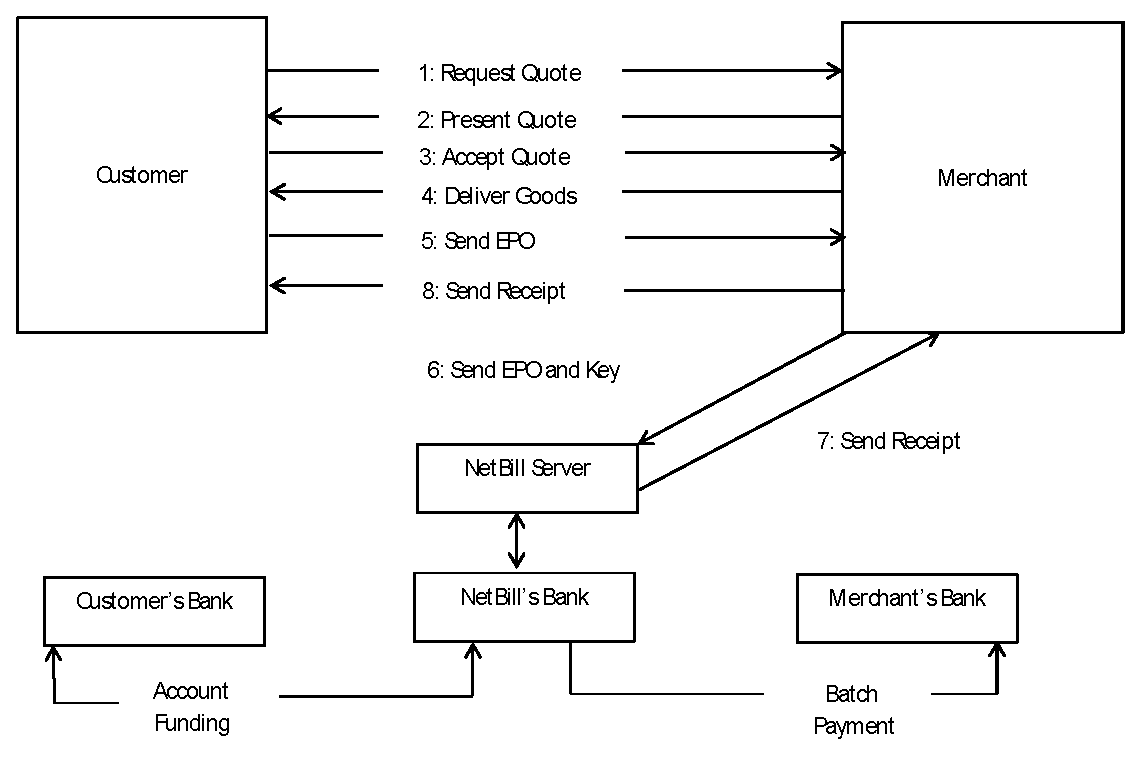
\includegraphics[width=12cm, height=8cm]{figures/figure1.eps}
        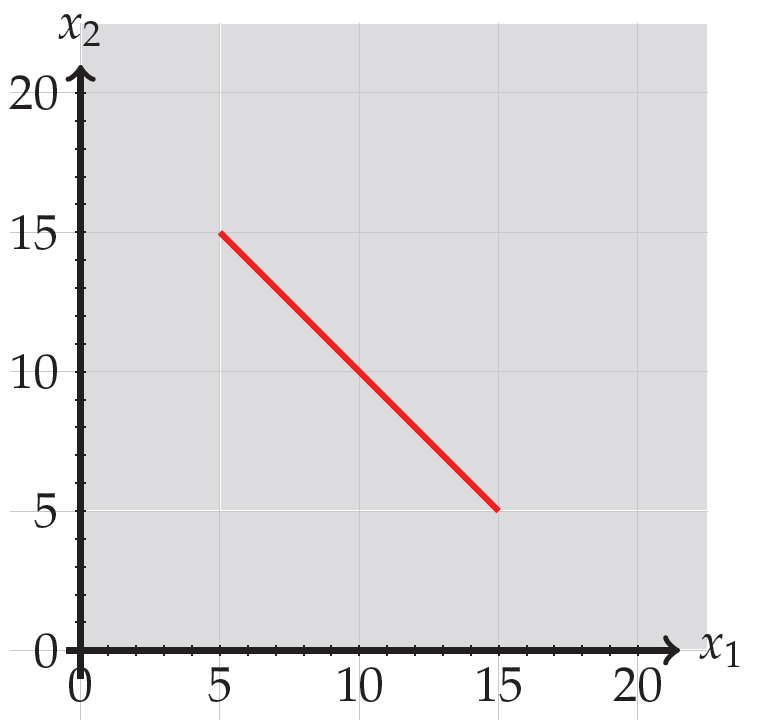
\includegraphics[width=0.3 \columnwidth]{figures/coreex1.png}
        %%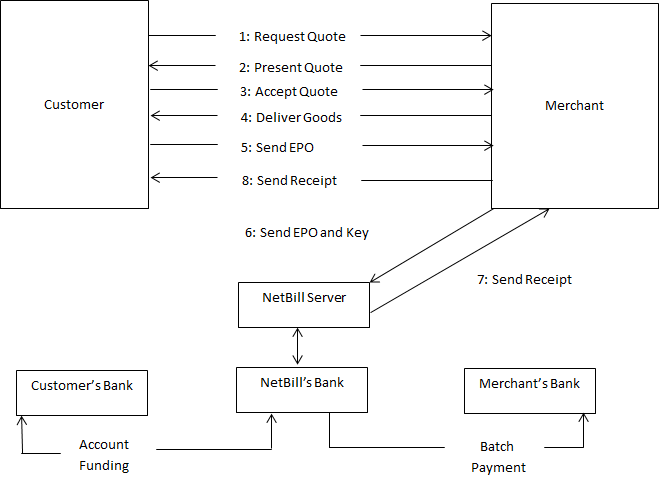
\includegraphics[scale=0.5]{figure1}
        %\caption{The NetBill payment protocol} \label{figure7}
    \end{figure}

    The core may not be fair: the core only considers stability.

\end{frame}

%%%%%%%%%%%%%%%%%%%%%%%%%%%%%%%%%%%%%%%%%%%%%%%%%%%%%%%%%%%%%%%%%%%%%%%%%%%%%%
\begin{frame} {Example 2: Three-player majority game}
    \begin{center}
      $N = \{1,2,3\}$ \\
      $v(\{i\}) = 0,$\\
      $v(\{C\}) = \alpha, for |C| = 2$ \\
      $v(N) = 1$ \\
    \end{center}
    \[ (x_1, x_2, x_3) \in Core(N,n) \iff \left\{
      \begin{array}{l l}
        x_i \geq 0 & \quad \forall i \in N\\
        x_i + x_j \geq \alpha & \quad \forall(i,j) \in N^2 i \neq j\\
        \sum_{i \in N} x_i = 1 &
      \end{array} \right.\]
    \[ (x_1, x_2, x_3) \in Core(N,n) \iff \left\{
      \begin{array}{l l}
        0 \leq x_i \leq 1 - \alpha & \quad \forall i \in N\\
        \sum_{i \in N} x_i = 1 &
      \end{array} \right.\]

    $Core(N,v)$ is nonempty $iff \alpha \leq \frac{2}{3}$ \\

    \begin{itemize}
        \item The core may not be fair: the core only considers stability. \\
        \item The core may not have an answer!
    \end{itemize}

\end{frame}
%%%%%%%%%%%%%%%%%%%%%%%%%%%%%%%%%%%%%%%%%%%%%%%%%%%%%%%%%%%%%%%%%%%%%%%%%%%%%
%%%%%%%%%%%%%%%%%%%%%%%%%%%%%%%%%%%%%%%%%%%%%%%%%%%%%%%%%%%%%%%%%%%%%%%%%%%%%
\section{Fairness and Shapley Value}
\subsection{Fairness and Shapley Value}

%%%%%%%%%%%%%%%%%%%%%%%%%%%%%%%%%%%%%%%%%%%%%%%%%%%%%%%%%%%%%%%%%%%%%%%%%%
\begin{frame}{Overview}
    \begin{itemize}
     	\itemsep=.5cm
    	\item Coalition Games
    	\item Stability and Core
    	\item {\bf Fairness and Shapley Value}
    	\item Other Solution Concepts
        \item Practical Example
    \end{itemize}
\end{frame}

%%%%%%%%%%%%%%%%%%%%%%%%%%%%%%%%%%%%%%%%%%%%%%%%%%%%%%%%%%%%%%%%%%%%%%%%%%%%%
\begin{frame}{Solution Concepts: Shapley Value}
    \begin{definition} [Marginal Contribution]\label{dfn:marginalcontribution}
        The {\color{blue}marginal contribution} of agent $i$ for a coalition $C \subseteq N \backslash \{i\}$ is $mc_i(C) = v(C \cup \{i\}) - v(C)$
    \end{definition}

    \begin{itemize}
        \item By considering average marginal contribution over all possible subsets of coalitions, we can achieve a fair distribution.\\
        \item Let $\prod(N)$ denote the set of all permutations of the sequence $(1,...n)$. Therefore: $\phi_i(N,v) = \frac{\sum_{\sigma \in \phi_i(N)}}{mc(\sigma)}$
    \end{itemize}

    \begin{definition} [Shapley Value]\label{dfn:shapleyvalue}
        Given a coalitional game $(N,v)$, the Shapley value of player $i$ is given by: \\
        $\phi_i(N,v) = \sum_{S \subseteq N \backslash \left\{i\right\} } \frac{|S|! (|N|-|S|-1)!}{|N|!} (v(S \cup \left\{i\right\}) - v(S))$
    \end{definition}
\end{frame}

%%%%%%%%%%%%%%%%%%%%%%%%%%%%%%%%%%%%%%%%%%%%%%%%%%%%%%%%%%%%%%%%%%%%%%%%%%%%%%
\begin{frame} {Example: Glove game}
    The {\color{blue}glove game} is a coalitional game where the players have left and right hand gloves and the goal is to form pairs
    \begin{center}
      $N = \{1,2,3\}$ \\
    \end{center}
    where players 1 and 2 have right hand gloves and player 3 has a left hand glove.
    \[ v(S) = \left\{
      \begin{array}{l l}
        1 & \quad if \quad S \in \{\{1,3\},\{2,3\},\{1,2,3\}\} \\
        0 & \quad otherwise
      \end{array} \right.\]
    $S = \emptyset, v(\{1\}) - v(\emptyset) = 0 - 0 = 0$ \\
    $S = \{2\}, v(\{1,2\}) - v(\{2\}) = 0 - 0 = 0$ \\
    $S = \{3\}, v(\{1,3\}) - v(\{3\}) = 1 - 0 = 1$ \\
    $S = \{2,3\}, v(\{1,2,3\}) - v(\{2,3\}) = 1 - 1 = 0$ \\
    \begin{itemize}
        \item ${\color{blue}x_1} = 0 + 0 + \frac{1}{6} + 0 = \frac{1}{6}$, ${\color{blue}x_2} = \frac{1}{6}$, ${\color{blue}x_3} = \frac{2}{3}$
        \item ${\color{blue}x} = (\frac{1}{6}, \frac{1}{6}, \frac{2}{3})$
    \end{itemize}
\end{frame}

%%%%%%%%%%%%%%%%%%%%%%%%%%%%%%%%%%%%%%%%%%%%%%%%%%%%%%%%%%%%%%%%%%%%%%%%%%%%%%%
\begin{frame}{Some Properties}
    \begin{itemize}
        \item The core may not always be non-empty.
        \item Shapley value always exists and is unique.
        \item When the valuation function is {\color{blue}superadditive}, the Shapley value is {\color{blue}individually rational}, i.e., it is an imputation.
        \item When the valuation function is {\color{blue}convex}, the Shapley value is also group rational, hence, it is in the {\color{blue}core}.
        \item A convex game has a non-empty core.
        \item Core and Shapley value are combinatorial problems.
        \item There are other well-known solution concepts: Bargaining set, nucleolus and kernel.
    \end{itemize}
\end{frame}

%%%%%%%%%%%%%%%%%%%%%%%%%%%%%%%%%%%%%%%%%%%%%%%%%%%%%%%%%%%%%%%%%%%%%%%%%%%%%
%%%%%%%%%%%%%%%%%%%%%%%%%%%%%%%%%%%%%%%%%%%%%%%%%%%%%%%%%%%%%%%%%%%%%%%%%%%%%
\section{Other Solution Concepts}
\subsection{Other Solution Concepts}

%%%%%%%%%%%%%%%%%%%%%%%%%%%%%%%%%%%%%%%%%%%%%%%%%%%%%%%%%%%%%%%%%%%%%%%%%%
\begin{frame}{Overview}
    \begin{itemize}
     	\itemsep=.5cm
    	\item Coalition Games
    	\item Stability and Core
    	\item Fairness and Shapley Value
    	\item {\bf Other Solution Concepts}
        \item Practical Example
    \end{itemize}
\end{frame}

%%%%%%%%%%%%%%%%%%%%%%%%%%%%%%%%%%%%%%%%%%%%%%%%%%%%%%%%%%%%%%%%%%%%%%%%%%%%%
\begin{frame}{$\epsilon$-Core}
    \begin{itemize}
        \item The core may not always be non-empty, core is a strong condition.
        \item $\epsilon$-core relaxes the core condition.
        \item $\forall S \subseteq N, \sum_{x_i \in S} x_i \geq v(S) - \epsilon$
        \item relative $\epsilon$-Core: $\forall S \subseteq N, \sum_{x_i \in S} x_i \geq (1-\epsilon).v(S)$
    \end{itemize}
\end{frame}

%%%%%%%%%%%%%%%%%%%%%%%%%%%%%%%%%%%%%%%%%%%%%%%%%%%%%%%%%%%%%%%%%%%%%%%%%%%%%
\begin{frame}{Excess of a coalition}
    \begin{itemize}
        \item We consider one way to compare two imputations.
    \end{itemize}

    \begin{definition} [Excess of a coalition]\label{dfn:marginalcontribution}
        Let (N,v) be a $TU$ game, $C \subseteq N$ be a coalition, and $x$ be a payoff distribution over $N$. The excess $e(C,x)$ of coalition $C$ at $x$ is the quantity $e(C,x) = v(C) - x(C)$.
    \end{definition}

    \begin{itemize}
        \item Example:
        \begin{itemize}
            \item let $N={1,2,3}, C={1,2}, v({1,2})=8, x=(3,2,5)$
            \item $e(C,x)=v({1,2})-(x_1 + x_2)=8-(3+2)=3.$
        \end{itemize}
    \end{itemize}

\end{frame}

%%%%%%%%%%%%%%%%%%%%%%%%%%%%%%%%%%%%%%%%%%%%%%%%%%%%%%%%%%%%%%%%%%%%%%%%%%%%%
\begin{frame}{Excess of a coalition}

    \begin{itemize}
        \item We can interpret a positive excess $(e(C,x) > 0)$ as the amount of dissatisfaction or {\color{blue} complaint} of the members of $C$ from the allocation x.
        \item We can use the excess to define the core:
        \begin{center}
            $Core(N,v)=\{x \in R^n |$ $x$ $is$ $an$ $imputation$ $and$ $\forall C \subseteq N, e(C,x) \leq 0\}$
        \end{center}
        \item This definition shows that no coalition has any complaint: each coalition's demand can be granted.
    \end{itemize}

\end{frame}

%%%%%%%%%%%%%%%%%%%%%%%%%%%%%%%%%%%%%%%%%%%%%%%%%%%%%%%%%%%%%%%%%%%%%%%%%%%%%
\begin{frame}{Excess of a coalition: Example}

    \centerline{$N = {1,2,3}$, $v(\{i\})=0$ $for$ $i \in \{1,2,3\}$ $v(\{1,2\}) = 5$}
    \centerline{$v(\{1,3\}) = 6$, $v(\{2,3\}) = 6$, $v(N) = 8$}

     \begin{itemize}
        \item Let us consider two payoff vectors $x = \{3, 3,2\}$ and $y = \{2, 3,3\}$.
        \item Let $e(x)$ denote the sequence of excesses of all coalitions at $x$.
     \end{itemize}


     \begin{table}[!htb]
        \begin{minipage}{.5\linewidth}
          \centering
            \begin{tabular}{c|c}
                \multicolumn{2}{c}{x = \{3,3,2\}} \\
                \hline
                \emph{Coalition C} & $e(C,x)$\\
                \hline
                \{1\} & -3\\
                \{2\} & -3\\
                \{3\} & -3\\
                \{1,2\} & -1\\
                \{1,3\} & 1\\
                \{2,3\} & 1\\
                \{1,2,3\} & 0\\
            \end{tabular}
        \end{minipage}%
        \begin{minipage}{.5\linewidth}
          \centering
            \begin{tabular}{c|c}
                \multicolumn{2}{c}{x = \{2,3,3\}} \\
                \hline
                \emph{Coalition C} & $e(C,x)$\\
                \hline
                \{1\} & -2\\
                \{2\} & -3\\
                \{3\} & -3\\
                \{1,2\} & 0\\
                \{1,3\} & 1\\
                \{2,3\} & 0\\
                \{1,2,3\} & 0\\
            \end{tabular}
        \end{minipage}
    \end{table}

\end{frame}

%%%%%%%%%%%%%%%%%%%%%%%%%%%%%%%%%%%%%%%%%%%%%%%%%%%%%%%%%%%%%%%%%%%%%%%%%%%%%
\begin{frame}{Excess of a coalition}
    \begin{itemize}
        \item Which payoff should we prefer? $x$ or $y$?
        \item Let us write the excess in the decreasing order (from the greatest excess to the smallest)
        \begin{itemize}
            \item $Sorted$ $e(C,x):$ $\{1, 1, 0,-1,-2,-3,-3\}$
            \item $Sorted$ $e(C,y):$ $\{1, 0, 0, 0,-2,-3,-3\}$
        \end{itemize}
    \end{itemize}

\end{frame}


%%%%%%%%%%%%%%%%%%%%%%%%%%%%%%%%%%%%%%%%%%%%%%%%%%%%%%%%%%%%%%%%%%%%%%%%%%%%%
\begin{frame}{Excess of a coalition: lexicographical order}

    \begin{definition} [lexicographical order $\geq_{lex}$]\label{dfn:lexorder}
        Let $\geq_{lex}$ denote the lexicographical ordering of $R^m$,
        $\forall(x,y) \in R^m, x \geq y$ $iff$
        \begin{itemize}
            \item $x=y$ or
            \item $\exists t$ $1 \leq t \leq m$ and $\forall i$ $1 \leq i < t$ $x_i = y_i$ and $x_t > y_t$
        \end{itemize}
    \end{definition}

    \begin{itemize}
        \item Example:
        \begin{itemize}
            \item let $\{1, 1, 0,-1,-2,-3,-3\} \geq_{lex} \{1, 0, 0, 0,-2,-3,-3\}$
        \end{itemize}
        \item Let $l$ be a sequence of $m$ reals. We denote by {\color{blue} $l^*$} the {\color{blue} reordering} of {\color{blue} $l$} in {\color{blue} decreasing} order.
        \item In the example, $e(x) = \{3,-3,-2,-1, 1, 1,0\}$ and then $e(x)^* = \{1, 1, 0,-1,-2,-3,-3\}$.
        \item Hence, we can say that $y$ is better than $x$ by writing $e(x)^* \geq e(y)^*$
    \end{itemize}

\end{frame}

%%%%%%%%%%%%%%%%%%%%%%%%%%%%%%%%%%%%%%%%%%%%%%%%%%%%%%%%%%%%%%%%%%%%%%%%%%%%%
\begin{frame}{Nucleolus}
    \begin{itemize}
        \item Let $(N,v)$ be a $TU$ game.
        \item Let $Imp$ be the set of all imputations.
        \item The {\color{blue}$nucleolus$ $Nu(N,v)$} is the set:
        \begin{itemize}
            \item $Nu(N,v) = \{x \in Imp | \forall y \in Imp, e(y)^* \geq_{lex} e(x)^*\}$
        \end{itemize}
    \end{itemize}
\end{frame}







%%%%%%%%%%%%%%%%%%%%%%%%%%%%%%%%%%%%%%%%%%%%%%%%%%%%%%%%%%%%%%%%%%%%%%%%%%%%%%%
\section{Practical Example}
\subsection{Problem Formulation and Modeling}


%%%%%%%%%%%%%%%%%%%%%%%%%%%%%%%%%%%%%%%%%%%%%%%%%%%%%%%%%%%%%%%%%%%%%%%%%%
\begin{frame}{Overview}
    \begin{itemize}
     	\itemsep=.5cm
    	\item Coalition Games
    	\item Stability and Core
    	\item Fairness and Shapley Value
    	\item Other Solution Concepts
        \item {\bf Practical Example}
    \end{itemize}
\end{frame}


\begin{frame}{Problem Formulation and Modeling}
    \begin{itemize}
        \item Communities of web services are robust service providers with well established market share and reputation.
        \item The community is characterized by a request rate $R_C$.
        \item Web services can perform tasks with some throughput rate ($Th_{ws}$).
        \item Web services come with different values of $QoS_{ws}$ for different metrics.
    \end{itemize}
\end{frame}

%%%%%%%%%%%%%%%%%%%%%%%%%%%%%%%%%%%%%%%%%%%%%%%%%%%%%%%%%%%%%%%%%%%%%%%%%%%%%%%
\begin{frame}{Task Distribution}
    \begin{itemize}
        \item Our model uses a slightly modified \emph{weighted fair queuing} method for task distribution rather than Contract-Net.
        \item All the input flow is multiplexed among different web services with weights proportional to their throughput value ($Th_{ws}$).
        \item Queues will happen if $R_C$ is more than the summation of web services throughput.
        \item Weighted task rate: $R_C \times \frac{Th_{ws}}{\sum_{ws}{Th_{ws}}}$ or $Th_{ws}$
    \end{itemize}
    \begin{figure}[htbp]
        \centering
        %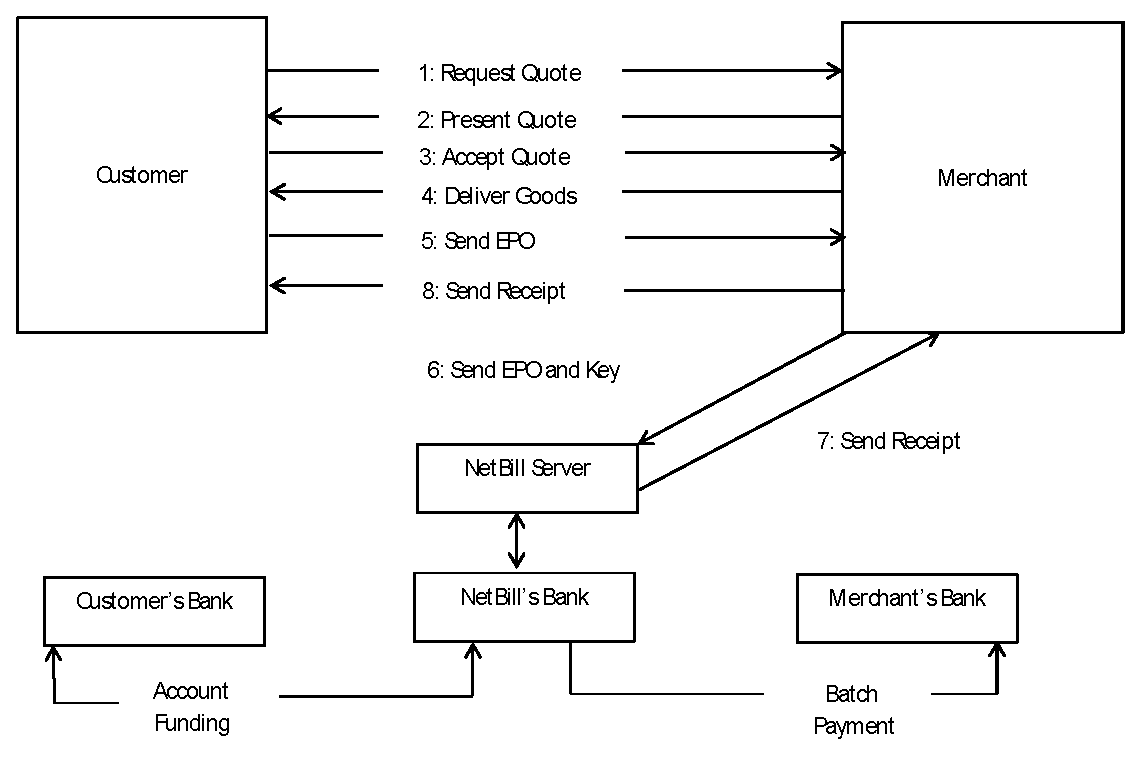
\includegraphics[width=12cm, height=8cm]{figures/figure1.eps}
        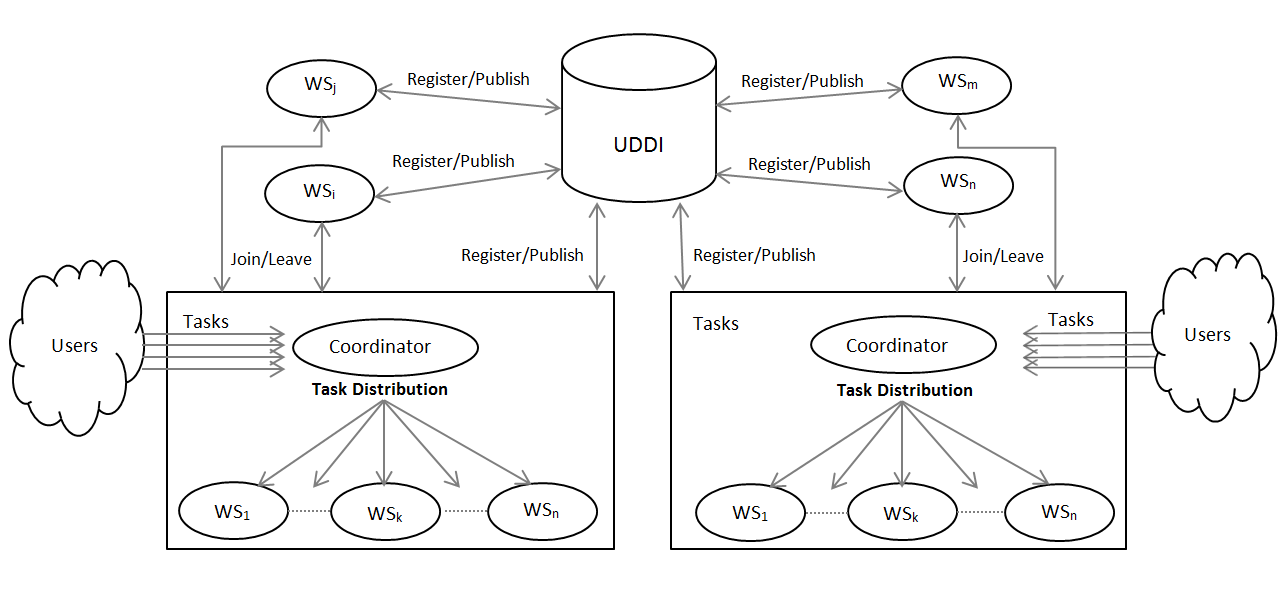
\includegraphics[width=0.8 \columnwidth]{figures/community.png}
        %%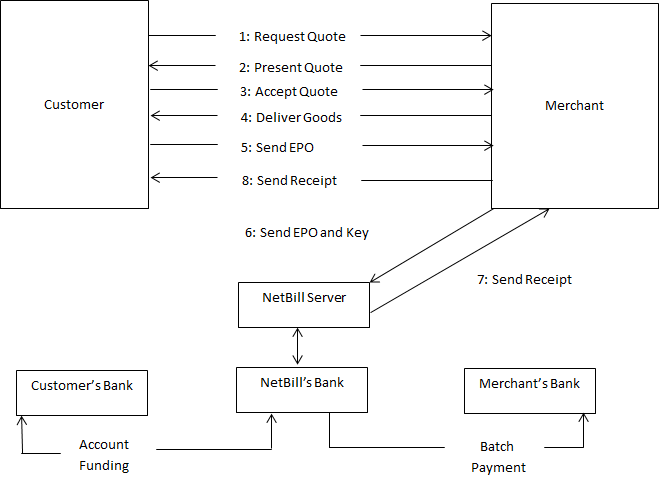
\includegraphics[scale=0.5]{figure1}
        %\caption{The NetBill payment protocol} \label{figure7}
    \end{figure}
\end{frame}

%%%%%%%%%%%%%%%%%%%%%%%%%%%%%%%%%%%%%%%%%%%%%%%%%%%%%%%%%%%%%%%%%%%%%%%%%%%%%%%
\begin{frame}{Community Revenue}
    \begin{itemize}
        \item Maximum potential output of a community:
            \begin{equation*}
                PO(C) = \sum_{ws \in C}{(T_{ws} \times QoS_{ws})}
            \end{equation*}
        \item if $\sum_{ws}{Th_{ws}} > R_C$, the community cannot perform at its maximum potential.
        \item Actual output:
            \begin{equation}\label{out_c}
                Out(C) = \left\{
                  \begin{array}{l l}
                    PO(C) & \quad \text{if $\sum_{ws}{Th_{ws}} \leq R_{C}$}\\
                    PO(C) \times \frac{R_{C}}{\sum_{ws}{Th_{ws}}} & \quad \text{if $\sum_{ws}{Th_{ws}} > R_{C}$}
                  \end{array} \right.
            \end{equation}
    \end{itemize}
\end{frame}

%%%%%%%%%%%%%%%%%%%%%%%%%%%%%%%%%%%%%%%%%%%%%%%%%%%%%%%%%%%%%%%%%%%%%%%%%%%%%%%
\begin{frame}{Example 1}
    \begin{table}[!t]
    \renewcommand{\arraystretch}{1.3}
    % if using array.sty, it might be a good idea to tweak the value of
    % \extrarowheight as needed to properly center the text within the cells
    \label{example_1}
    \centering
    \begin{tabular}{c c c c}
    \hline
    $WS$ & $QoS_{ws}$ & $Th_{ws}$ & $Th_{ws} \times QoS_{ws}$\\
    \hline
    1 & 0.8 & 4 & 3.2\\
    2 & 0.8 & 5 & 4.0\\
    3 & 0.8 & 3 & 2.4\\
    \hline
    \end{tabular}
    \end{table}

    \begin{table}[!t]
    \renewcommand{\arraystretch}{1.3}
    % if using array.sty, it might be a good idea to tweak the value of
    % \extrarowheight as needed to properly center the text within the cells
    % \caption{Three web services}
    \label{example_1_2}
    \centering
    \begin{tabular}{c c || c c}
    \hline
    Community & Worth & Community & Worth\\
    \hline
    $\left\{1\right\}$ & 3.2 & $\left\{1,2\right\}$ & 7.2\\
    $\left\{2\right\}$ & 4.0 & $\left\{1,3\right\}$ & 5.6\\
    $\left\{3\right\}$ & 2.4 & $\left\{2,3\right\}$ & 6.4\\
    $\left\{1,2,3\right\}$ & 8.0\\
    \hline
    Community $R_C$: 10\\
    \hline
    \end{tabular}
    \end{table}
\end{frame}

%%%%%%%%%%%%%%%%%%%%%%%%%%%%%%%%%%%%%%%%%%%%%%%%%%%%%%%%%%%%%%%%%%%%%%%%%%%%%%%%
%\begin{frame}{Example 2}
%    \begin{table}[!t]
%    \renewcommand{\arraystretch}{1.3}
%    % if using array.sty, it might be a good idea to tweak the value of
%    % \extrarowheight as needed to properly center the text within the cells
%    \label{example_2}
%    \centering
%    \begin{tabular}{c c c c}
%    \hline
%    $WS$ & $QoS_{ws}$ & $Th_{ws}$ & $Th_{ws} \times QoS_{ws}$\\
%    \hline
%    1 & 0.8 & 5 & 4.0\\
%    2 & 0.7 & 6 & 4.2\\
%    3 & 0.7 & 4 & 2.8\\
%    \hline
%    \end{tabular}
%    \end{table}
%
%    \begin{table}[!t]
%    \renewcommand{\arraystretch}{1.3}
%    % if using array.sty, it might be a good idea to tweak the value of
%    % \extrarowheight as needed to properly center the text within the cells
%    % \caption{Three web services}
%    \label{example_2_2}
%    \centering
%    \begin{tabular}{c c || c c}
%    \hline
%    Community & Worth & Community & Worth\\
%    \hline
%    $\left\{1\right\}$ & 4.0 & $\left\{1,2\right\}$ & 7.4\\
%    $\left\{2\right\}$ & 4.2 & $\left\{1,3\right\}$ & 6.8\\
%    $\left\{3\right\}$ & 2.8 & $\left\{2,3\right\}$ & 7.0\\
%    $\left\{1,2,3\right\}$ & 7.3\\
%    \hline
%    Community $R_C$: 10\\
%    \hline
%    \end{tabular}
%    \end{table}
%\end{frame}

%%%%%%%%%%%%%%%%%%%%%%%%%%%%%%%%%%%%%%%%%%%%%%%%%%%%%%%%%%%%%%%%%%%%%%%%%%%%%%%
\begin{frame}{Example 2}
    \begin{table}[!t]
    \renewcommand{\arraystretch}{0.8}
    % if using array.sty, it might be a good idea to tweak the value of
    % \extrarowheight as needed to properly center the text within the cells
    \label{example_3}
    \centering
    \begin{tabular}{c c c c}
    \hline
    $WS$ & $QoS_{ws}$ & $Th_{ws}$ & $\text{\emph{Input Task Rate}}$\\
    \hline
    1 & 0.8 & 10 & 5\\
    2 & 0.8 & 20 & 5\\
    3 & 0.8 & 30 & 5\\
    \hline
    \end{tabular}
    \end{table}

    \begin{table}[!t]
    \renewcommand{\arraystretch}{0.8}
    % if using array.sty, it might be a good idea to tweak the value of
    % \extrarowheight as needed to properly center the text within the cells
    % \caption{Three web services}
    \label{example_3_2}
    \centering
    \begin{tabular}{c c || c c}
    \hline
    Community & Worth & Community & Worth\\
    \hline
    $\left\{C_{ms_1}\right\}$ & 0 & $\left\{C_{ms_2}\right\}$ & 0\\
    $\left\{C_{ms_1}, ws_1\right\}$ & 8 & $\left\{C_{ms_2}, ws_1\right\}$ & 8\\
    $\left\{C_{ms_1}, ws_2\right\}$ & 16 & $\left\{C_{ms_2}, ws_2\right\}$ & 16\\
    $\left\{C_{ms_1}, ws_3\right\}$ & 16 & $\left\{C_{ms_2}, ws_3\right\}$ & 24\\
    $\left\{C_{ms_1}, ws_1, ws_2\right\}$ & 16 & $\left\{C_{ms_2}, ws_1, ws_2\right\}$ & 24\\
    $\left\{C_{ms_1}, ws_1, ws_3\right\}$ & 16 & $\left\{C_{ms_2}, ws_1, ws_3\right\}$ & 32\\
    $\left\{C_{ms_1}, ws_2, ws_3\right\}$ & 16 & $\left\{C_{ms_2}, ws_2, ws_3\right\}$ & 32\\
    $\left\{C_{ms_1}, ws_1, ws_2, ws_3\right\}$ & 16 & $\left\{C_{ms_2}, ws_1, ws_2, ws_3\right\}$ & 32\\
    $\left\{C_{ms_1}, C_{ms_2}, ...\right\}$ & 0 & $\left\{ws_1\right\}$ & 6.8\\
    $\left\{ws_2\right\}$ & 4.2 & $\left\{ws_3\right\}$ & 6.8\\
    \hline
    Community $R_{C_1}$: 20 \\ Community $R_{C_2}$: 40\\
    \hline
    \end{tabular}
    \end{table}
\end{frame}

%%%%%%%%%%%%%%%%%%%%%%%%%%%%%%%% frame19 Proposed Research
%%%%%%%%%%%%%%%%%%%%%%%%%%%%%%%%%%%%%%%%%%%%%%%%%%%%%%%%%%%%%%%%%%%%%%%%%%%%%%%
\subsection{Web Service Cooperative Games}

%%%%%%%%%%%%%%%%%%%%%%%%%%%%%%%%%%%%%%%%%%%%%%%%%%%%%%%%%%%%%%%%%%%%%%%%%%%%%%%
\begin{frame}{Community and Web Service Interaction Model}
    \begin{figure}[htbp]
        \centering
        %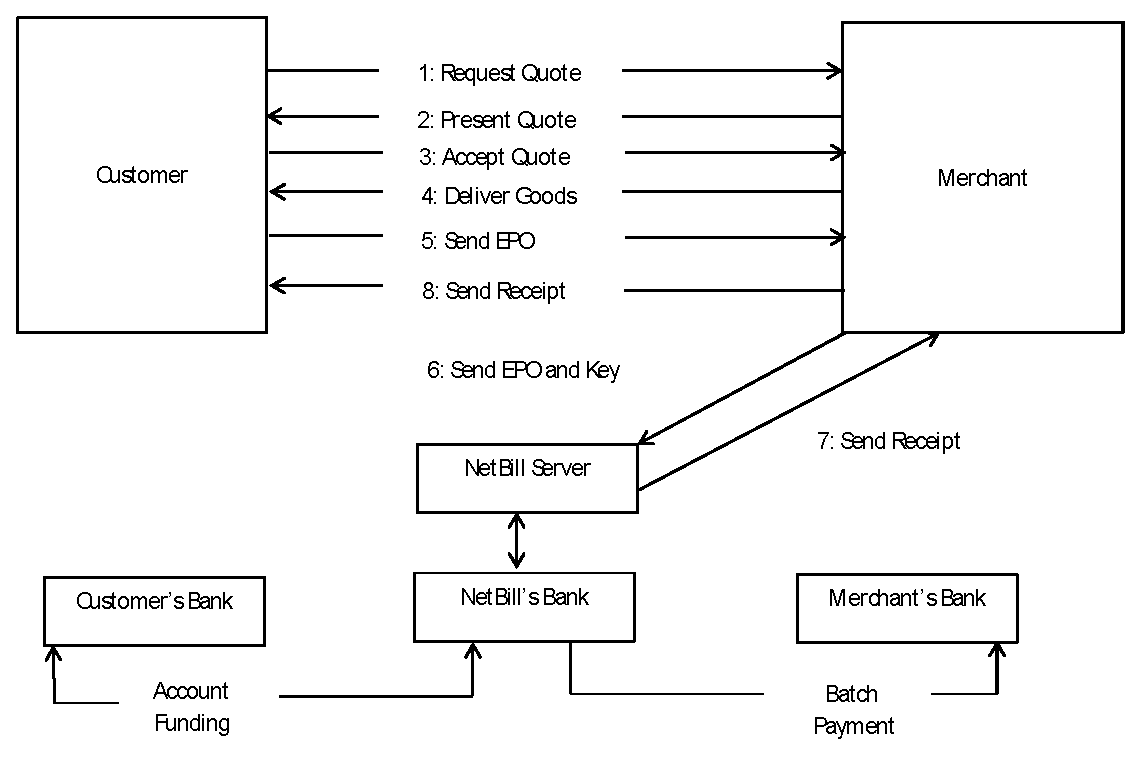
\includegraphics[width=12cm, height=8cm]{figures/figure1.eps}
        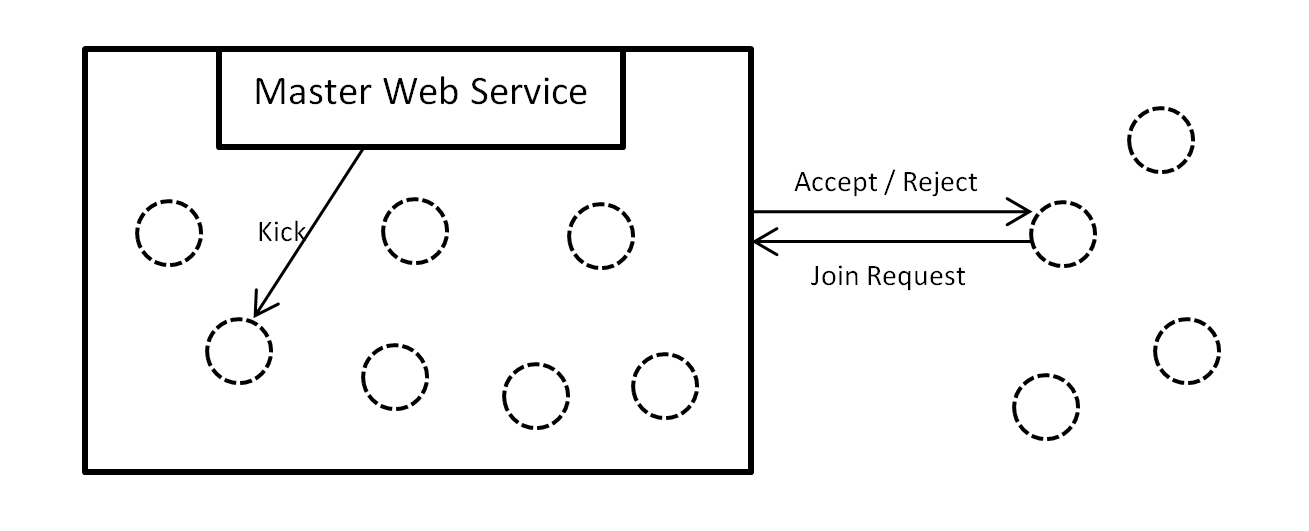
\includegraphics[width=0.8 \columnwidth]{figures/scenario1.png}
        %%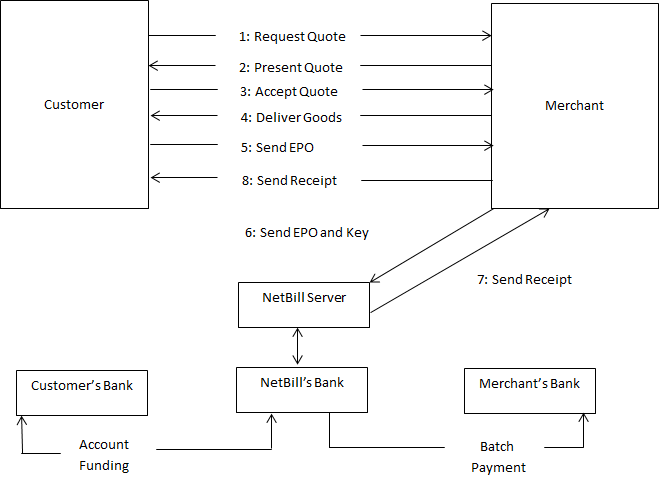
\includegraphics[scale=0.5]{figure1}
        %\caption{The NetBill payment protocol} \label{figure7}
    \end{figure}

    \begin{itemize}
        \item A typical WS community, where web services can join or leave.
        \item $v(C) = Out(C)$.
        \item Membership decision in made based on throughput and QoS of the web services.
        \item Community master needs to get quality web services to keep the community stable, so other web services have no incentive to leave.
    \end{itemize}
       	
\end{frame}
%%%%%%%%%%%%%%%%%%%%%%%%%%%%%%%%%%%%%%%%%%%%%%%%%%%%%%%%%%%%%%%%%%%%%%%%%%%%%%%
\begin{frame}{Community and Web Service Interaction Model}


    \begin{itemize}
        \item Upon receiving membership request, the master web service checks if the coalition will be stable having the new member.
        \item If the game is convex, core exists.
        \item If the game is convex, Shapley value is in core.
        \item Convexity Condition:
        \begin{center}
          $v(A \cup B) \geq v(A) + v(B) - v(A \cap B)$ \\
          $\Leftrightarrow$  \\
          $\forall S,T | S \subseteq T \subseteq N \backslash \left\{i\right\}, \forall i \in N,$ \\
          {\color{blue} $v(S \cup \left\{i\right\}) - v(S) \leq v (T \cup \left\{i\right\}) - v(T)$ }
        \end{center}
        \item Depth-1 Convexity Check: $O(n)$
        \item Depth-2 Convexity Check: $O(n^2)$
    \end{itemize}
       	
\end{frame}







\begin{frame}{Experimental Results}

    \begin{figure}[!t]
    \centering
    %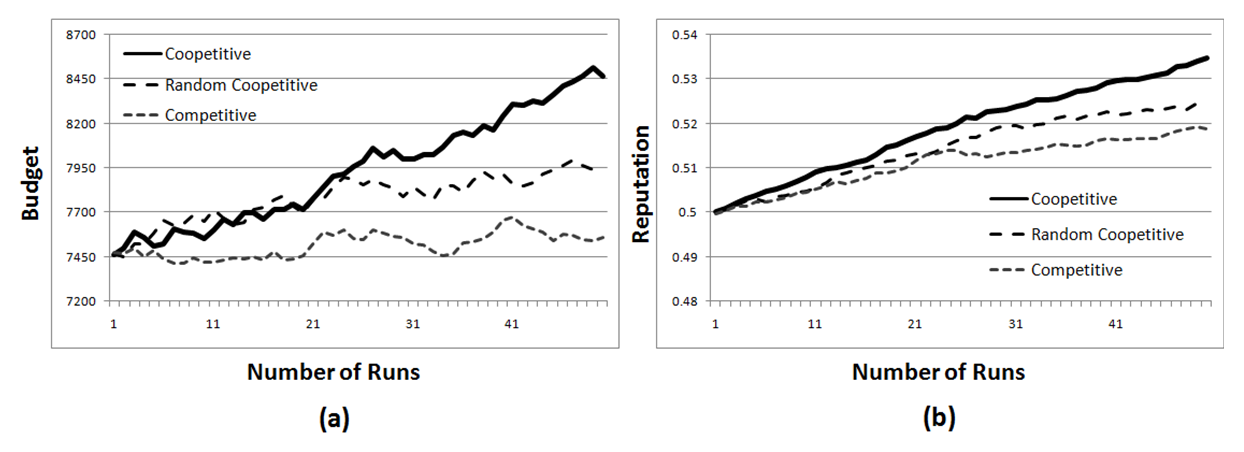
\includegraphics[scale=0.6]{graph1Final+.eps}
    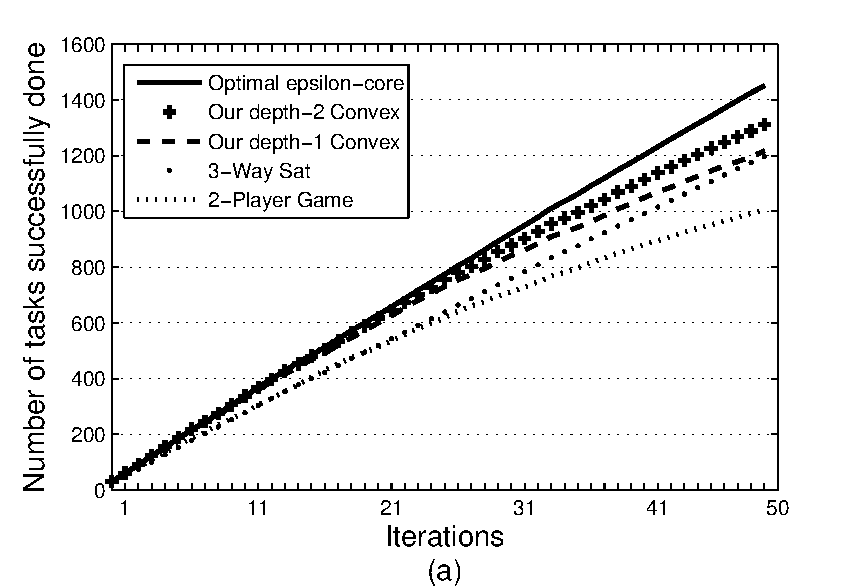
\includegraphics[width=2.1in]{figures/task_done_opt-eps-converted-to.pdf}
    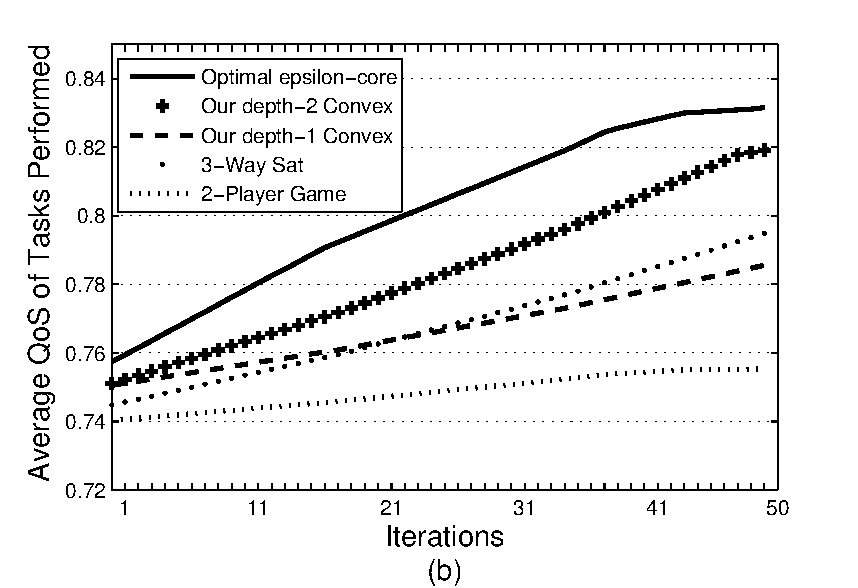
\includegraphics[width=2.1in]{figures/task_qos_opt-eps-converted-to.pdf}
    \caption{Part (a): Cumulative number of requests successfully
    answered. Part (b): Average QoS of requests performed.}
    \label{performanceall}
    \end{figure}

\end{frame}
%%%%%%%%%%%%%%%%%%%%%%%%%%%%%%%%%%%%%%%%%%%%%%%%%%%%%%%%%%%%%%%%%%%%%%%%%%%%%%

%%%%%%%%%%%%%%%%%%%%%%%%%%%%%%%%%%%%%%%%%%%%%%%%%%%%%%%%%%%%%%%%%%%%%%%%%%%%%%%
\begin{frame}{Improving Community Stability}
    \begin{itemize}
        \item The core may not always be non-empty, core is a strong condition.
        \item The optimal solution concepts will attract only enough services satisfying input task rate, not more.
        \item In case of web service failure, a portion of tasks will not be handled efficiently until replacement is found.
        \item By imposing cost on deviation or subsiding the community, its possible to attract more web services and keep the community stable.
        \item Will be cost efficient in case of web service failure, or for replacing web services dropping in QoS metrics as they advertised.
        \item \emph{Taxation} would need agreement between all communities (needs a centralized approach), however \emph{subsiding} can be done within communities in distributed manner.
    \end{itemize}
\end{frame}
%%%%%%%%%%%%%%%%%%%%%%%%%%%%%%%%%%%%%%%%%%%%%%%%%%%%%%%%%%%%%%%%%%%%%%%%%%%%%%%

%%%%%%%%%%%%%%%%%%%%%%%%%%%%%%%%%%%%%%%%%%%%%%%%%%%%%%%%%%%%%%%%%%%%%%%%%%%%%%%
\begin{frame}{Taxation and Subsiding}
    \begin{itemize}
        \item Least Core
        \begin{itemize}
            \item $\forall S \subseteq N, \sum_{x_i \in S} x_i \geq v(S) - \epsilon$
            \item $\epsilon$-core relaxes the core condition.
        \end{itemize}
        \item Taxation in Reliability Games \small $[Y. Bachrach, E. Elkind, 2009]$

        \item Taxation and Cost of Stability \small $[R. Meir, J. S. Rosenchein, 2011]$

        \item Taxation in Anonymous Games \small $[Y. Zick, M. Polukarov, 2013]$

        \item Relative Core
        \begin{itemize}
            \item $\lambda v(C)$ is divided among players.
            \item relative $\lambda$-Core: $\forall S \subseteq N, \sum_{x_i \in S} x_i \geq \frac{1}{\lambda}.v(S)$
            \item Clearly any community can be stabilized by large enough $\lambda$, however the community coordinator would be interested in the minimal subsidy required to stabilize the game.
            \item Can be solved using $LP$ if $v(S)$ is a linear function
        \end{itemize}
    \end{itemize}
\end{frame}
%%%%%%%%%%%%%%%%%%%%%%%%%%%%%%%%%%%%%%%%%%%%%%%%%%%%%%%%%%%%%%%%%%%%%%%%%%%%%%%

%%%%%%%%%%%%%%%%%%%%%%%%%%%%%%%%%%%%%%%%%%%%%%%%%%%%%%%%%%%%%%%%%%%%%%%%%%%%%%
\begin{frame}{Results: Taxation and Subsiding}
    \begin{figure}[!t]
        \centering
        %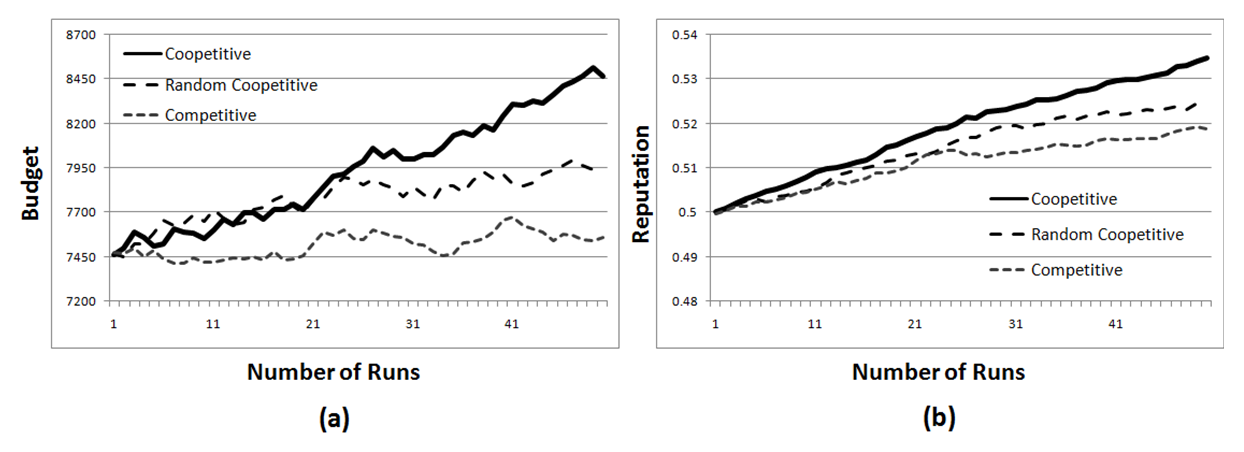
\includegraphics[scale=0.6]{graph1Final+.eps}
        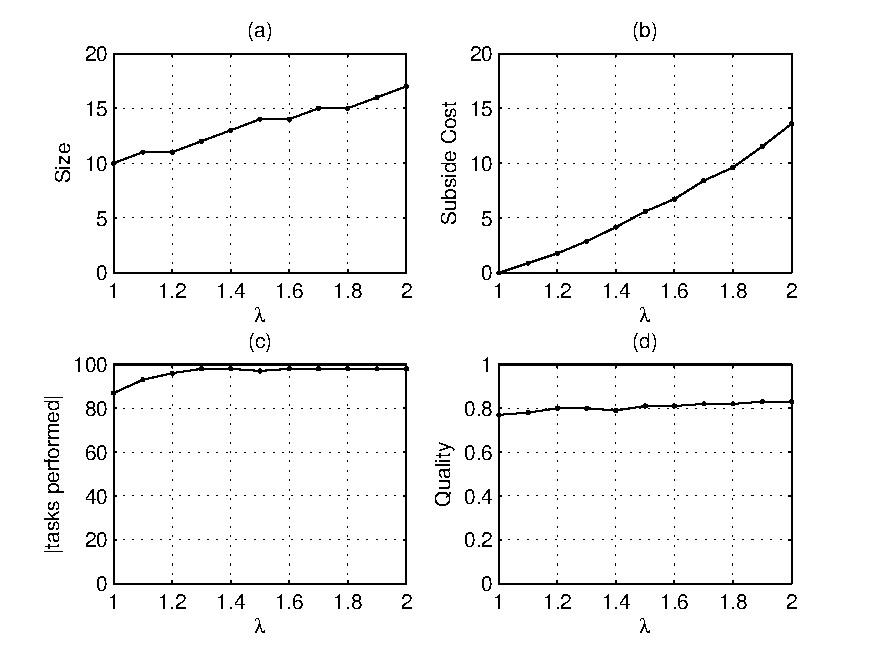
\includegraphics[width=3in]{figures/taxtation-eps-converted-to.pdf}
        \caption{Analysis of community subsiding coefficient $\lambda$ on
        average community size (a), cost (b), number of tasks performed
        (c), and average quality of service of tasks performed (d).}
        \label{f_taxtation}
    \end{figure}
\end{frame}
%%%%%%%%%%%%%%%%%%%%%%%%%%%%%%%%%%%%%%%%%%%%%%%%%%%%%%%%%%%%%%%%%%%%%%%%%%%%%%

%%%%%%%%%%%%%%%%%%%%%%%%%%%%%%%%%%%%%%%%%%%%%%%%%%%%%%%%%%%%%%%%%%%%%%%%%%%%%%
\begin{frame}{Results: Taxation and Subsiding}
    \begin{figure}[!t]
        \centerline{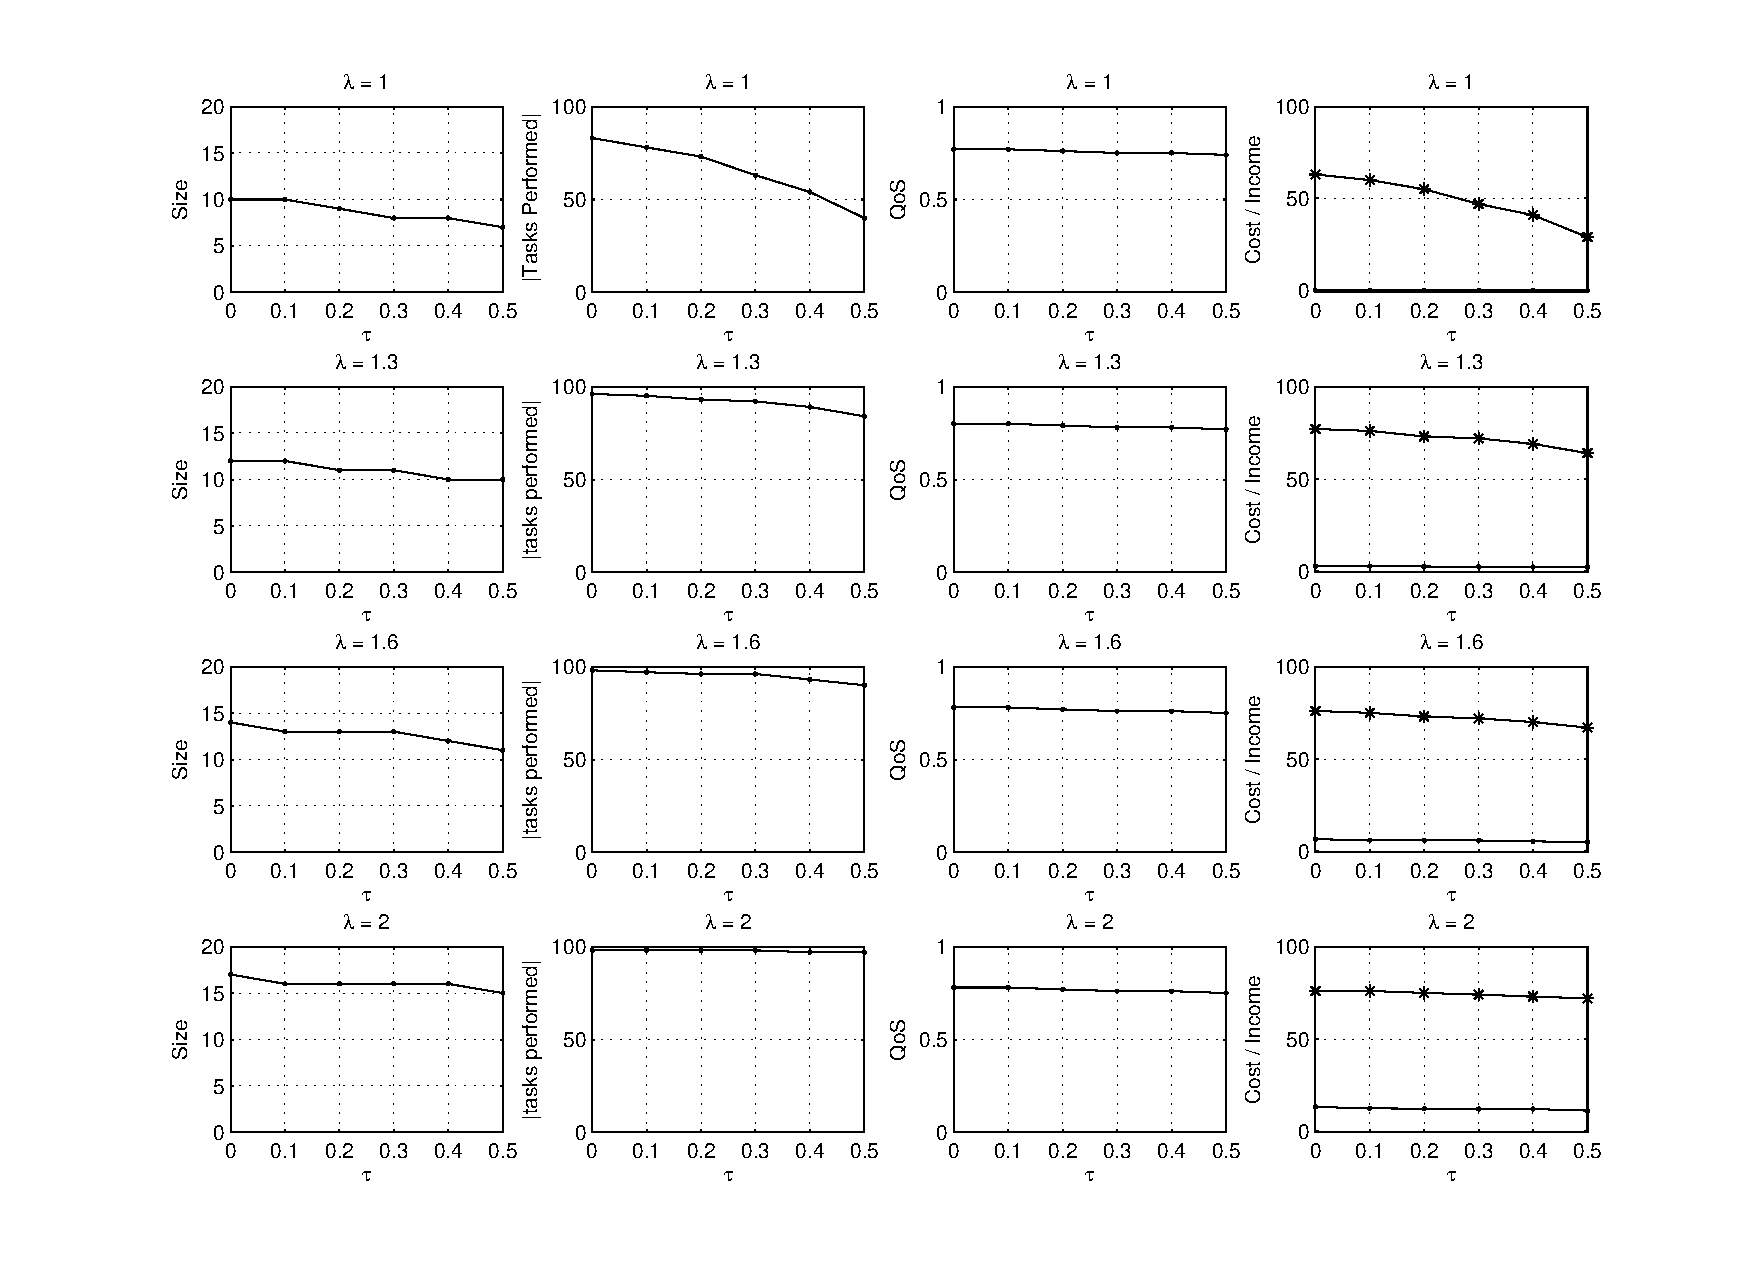
\includegraphics[width=4.2in]{figures/tax_dyn-eps-converted-to.pdf}}
        \caption{Analysis of community subsiding coefficient $\lambda$
        having web service different stability levels of $\tau$ on average
        community size, number of tasks performed, average quality of
        service, and average cost/income of communities.}
        \label{fig_dynamic_taxtation}
    \end{figure}
\end{frame}
%%%%%%%%%%%%%%%%%%%%%%%%%%%%%%%%%%%%%%%%%%%%%%%%%%%%%%%%%%%%%%%%%%%%%%%%%%%%%%





\end{document}
